\documentclass[handout, aspectratio = 169]{beamer}
%\documentclass[presentation]{beamer}

%https://www.overleaf.com/project/5f638086f8e558000137cf72

\usecolortheme{Imperial}
 
\usepackage[utf8]{inputenc}
\usepackage[UKenglish]{babel}
\usepackage{booktabs}
\usepackage{caption}
\usepackage{subcaption}
\usepackage{graphicx}
\usepackage{amsmath}
\usepackage{amsfonts}
\usepackage{amssymb}
\usepackage{epstopdf}
\usepackage{animate}
\usepackage{fancyvrb}

% complying UK date format, i.e. 1 January 2001
\usepackage{datetime}
\let\dateUKenglish\relax
\newdateformat{dateUKenglish}{\THEDAY~\monthname[\THEMONTH] \THEYEAR}

% Imperial College Logo, not to be changed!
\institute{
\includegraphics[height=0.7cm]{Imperial_1_Pantone_solid.eps}}



% -----------------------------------------------------------------------------

\setbeamertemplate{itemize items}[triangle]
\setbeamertemplate{enumerate items}[circle]

%\graphicspath{{figures/}}

%Information to be included in the title page:
\title{Machine Learning Workshop}

%\subtitle{Subtitle}

\author{\color{black} \textbf{Tim C.D. Lucas}\\
{\color{white}blank}\\

\includegraphics[height=7pt]{Ar_Icon_Contact.pdf} tlucas{\footnotesize{@}}ic.ac.uk}

\date{\today}



\begin{document}
 
\frame{\titlepage

% pushes logo up a little but doesn't affect blue line.
\vspace{-0.2cm}
\hfill % pushes logo the right
\includegraphics[width=5cm]{../../ceh_logo.png}

}



%plan:

%1 what is ml 
%what models count
%2 tasks
% famous examples
%4 fit rpart in caret
%- the data
%- hold out
%- error metric
%3 what is caret and it helps an interface with %those many different models


%5 what is ml good at
%compare lm and RF in simplest caret

%6 what is ml bad at
%compare RF and Newton on planets and gravity
%uncertainty

%7 tuning parameters.
%7 very flexible models
%do x^6
%overfitting
%8 bias variance
%9 we might call 6 a hyperparameter.
%lots of models have hyperparameters that %control how regularised the model is.

%10 how do we choose it?
%use hold out data
%CV
%Caret tune parameter

%11 inner outer. use outer for main research %question. which model is best or how well will %my model work in the real world.

%13 match error metric to question


%12 a full machine learning workflow.


%extras:


%14 ask questions with cv
%15-17 trees, RF, enet in a bit more detail. nnet.
%18 no free lunch. try lots of models


\begin{frame}
\frametitle{What is machine learning?}
\begin{itemize}
\item Focus on prediction
\item Not mechanistic/process based models
\item Not inference of real-world parameters.
\end{itemize}
\end{frame} 


\begin{frame}
\frametitle{What is machine learning?}
\begin{enumerate}
\item Parametric, statistical 
\begin{itemize}
\item Linear regression, LASSO.
\end{itemize}

\item Nonparametric, statistical.
\begin{itemize}
\item Gaussian processes, splines.
\end{itemize}
\item Nonparametric, nonstatistical.
\begin{itemize}
\item Neural networks, decision trees, random forest.
\end{itemize}
\end{enumerate}
\end{frame} 

\begin{frame}[fragile]
\frametitle{Let's do Machine Learning: Data}
Time until death data
\begin{Verbatim}

data(melanoma, package = "boot")

head(melanoma)

featurePlot(melanoma[, -1], 
                     melanoma$time)

\end{Verbatim}

\end{frame} 

\begin{frame}[fragile]
\frametitle{ Let's do Machine Learning: Training a model}
\begin{Verbatim}

m0 <- train(time ~ ., 
            data = melanoma,
            method = 'rpart2')

\end{Verbatim}

\end{frame} 



\begin{frame}
\frametitle{Any questions?}

(This slide will occur many times in this slidedeck.

\end{frame} 



\begin{frame}
\frametitle{Look at learned model}
\vspace{-4mm}
\begin{figure}
    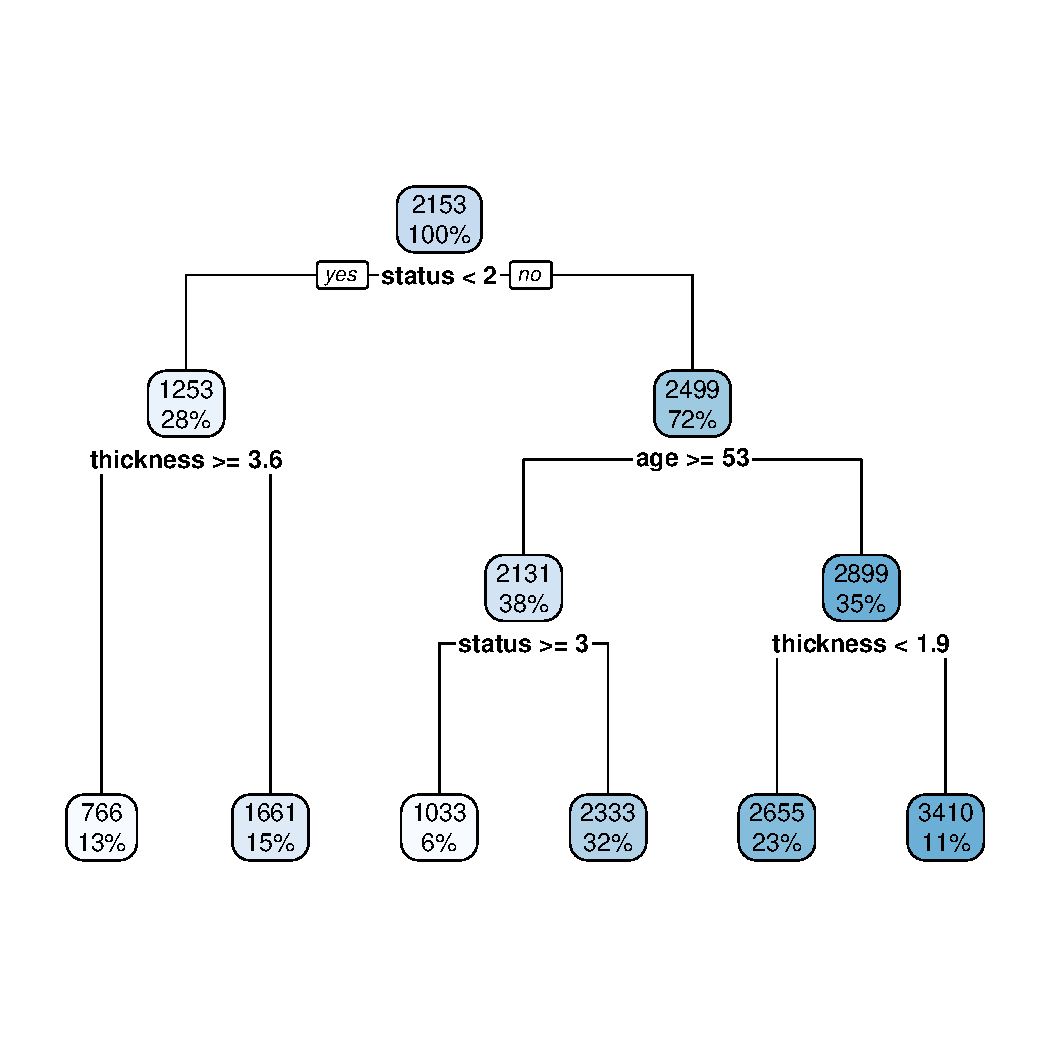
\includegraphics[width = 0.5\textwidth]{rpart_tree.pdf}
\end{figure} 

\end{frame} 



\begin{frame}
\frametitle{Look at learned model}
\vspace{2mm}
\begin{figure}
    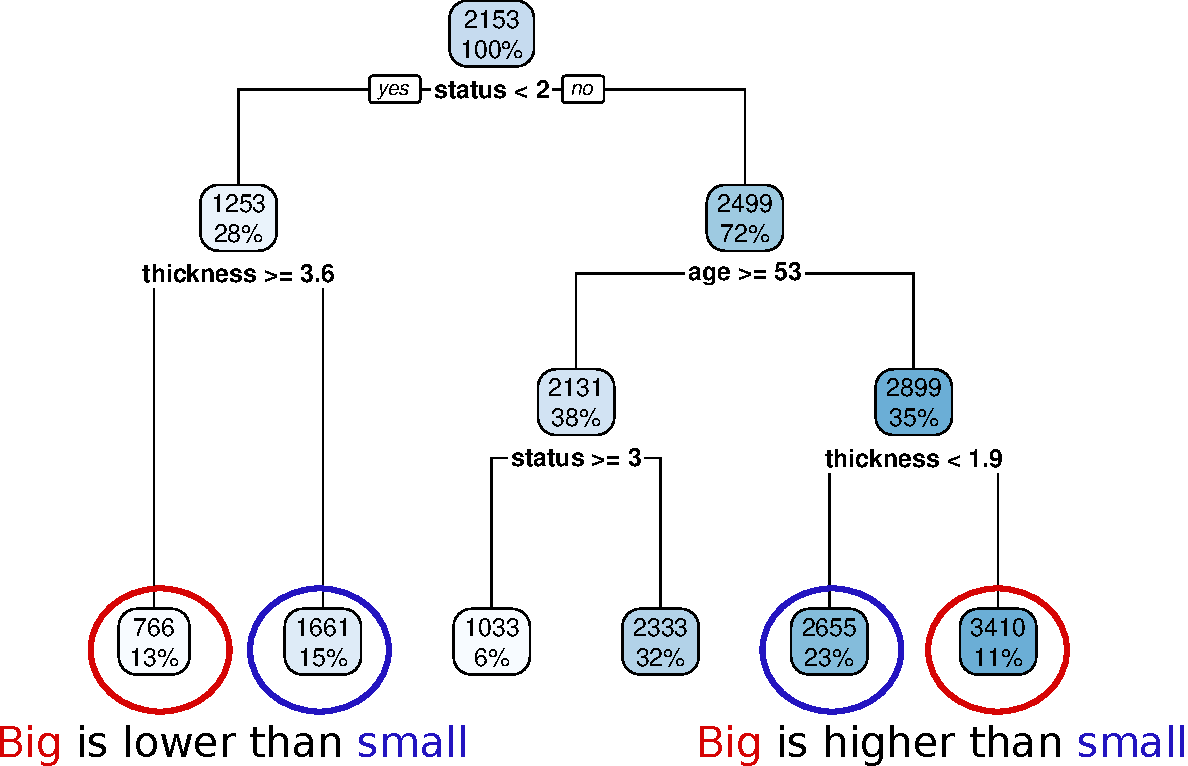
\includegraphics[width = 0.6\textwidth]{rpart_annotate.pdf}
\end{figure} 

\end{frame} 




\begin{frame}
\frametitle{What is machine learning?}
Supervised learning.

Classification or regression.
\begin{figure}
    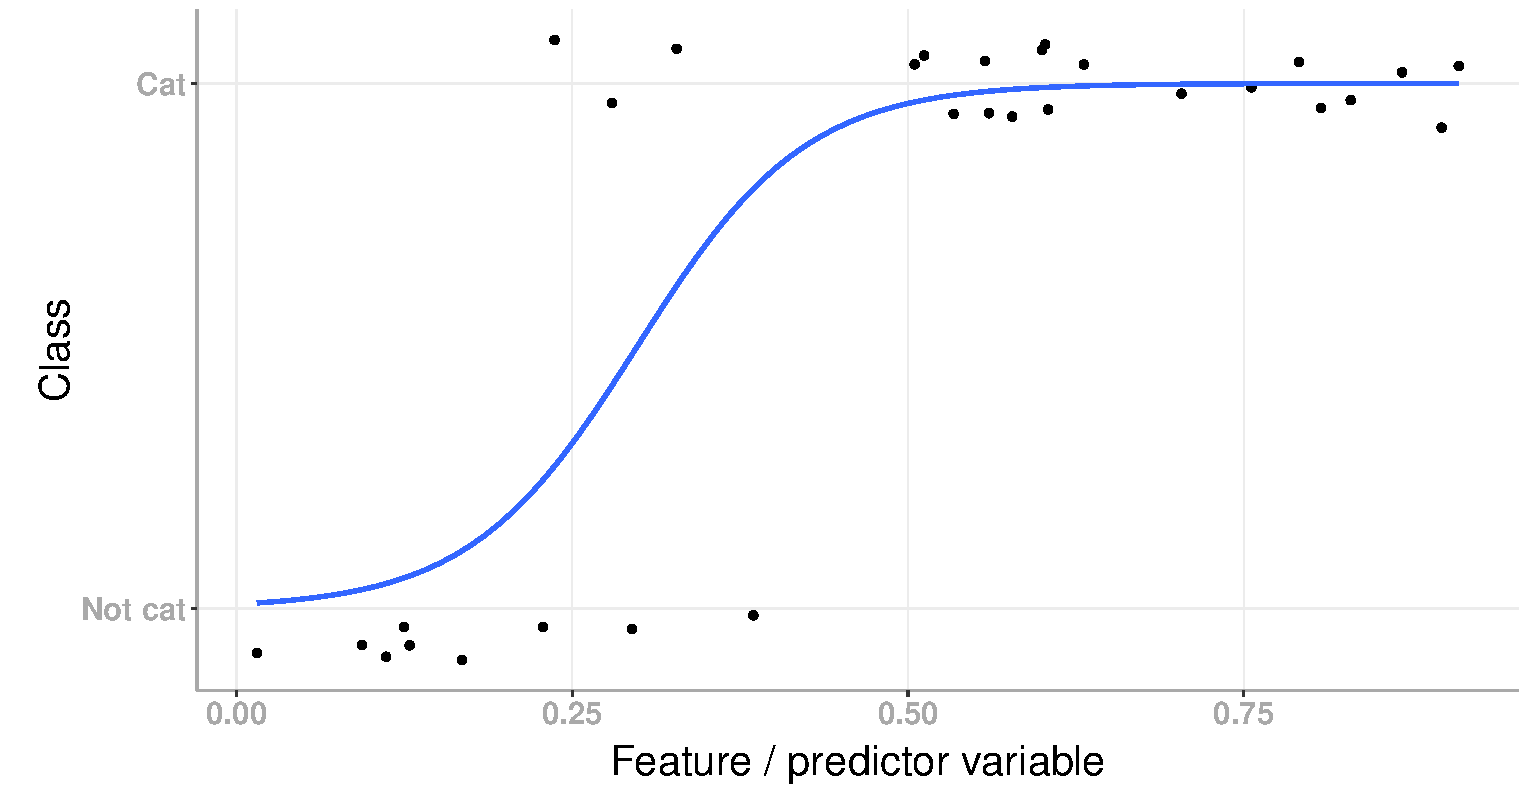
\includegraphics[width = 0.5\textwidth]{classification}%
    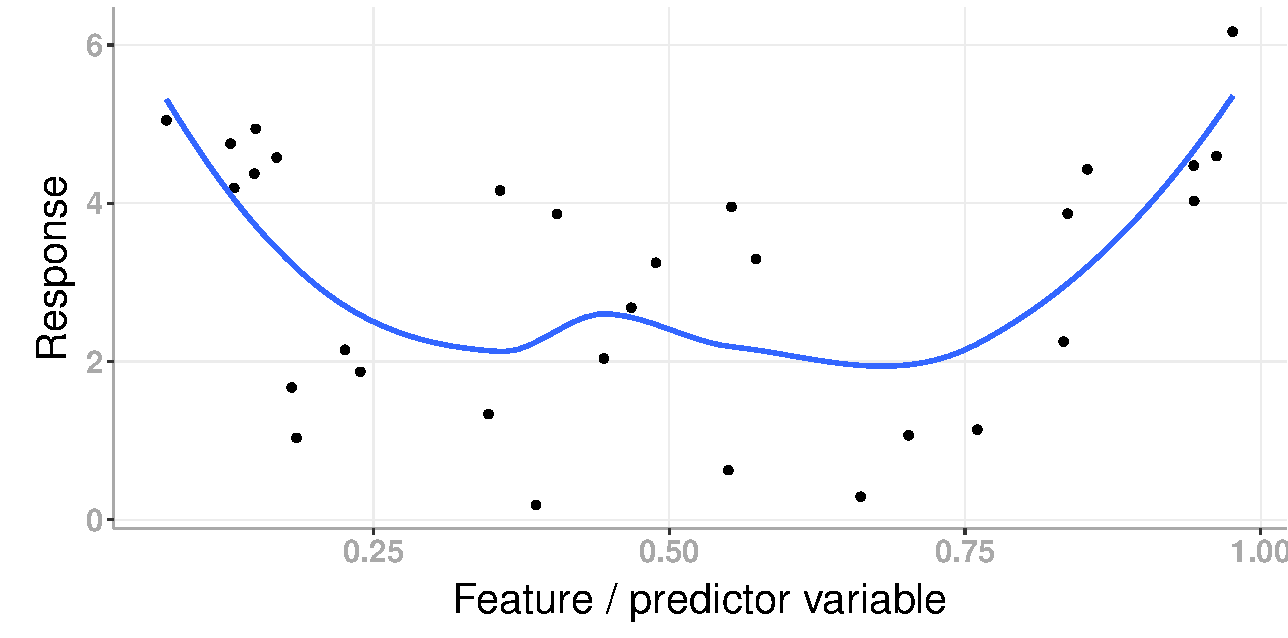
\includegraphics[width = 0.5\textwidth]{regression}
\end{figure} 

\end{frame} 


\begin{frame}
\frametitle{Caret package}
\begin{itemize}
\item https://topepo.github.io/caret/model-training-and-tuning.html
\item Unified interface to hundreds of models
\item Supervised learning
\item Full ML workflow
\item Excellent documentation
\end{itemize}

\end{frame} 



\begin{frame}
\frametitle{Any questions?}


\end{frame} 


\begin{frame}
\frametitle{What is machine learning?}
Other tasks:
\begin{itemize}
\item Reinforcement learning
\begin{itemize}
\item Make your own data.
\end{itemize}
\item Unsupervised learning
\begin{itemize}
\item Clustering.
\end{itemize}
\end{itemize}
\end{frame} 











\begin{frame}[fragile]
\frametitle{What is ML good at? Predicting new data.}
\renewcommand{\FancyVerbFormatLine}[1]{%
   \ifnum\value{FancyVerbLine}=8\color{cyan}#1%
   \else #1\fi}
\begin{Verbatim}
tr <- trainControl(
        method = 'LGOCV',
        number = 1)

m1 <- train(time ~ ., 
            data = melanoma,
            method = 'rpart2',
            trControl = tr)

\end{Verbatim}

\end{frame} 






\begin{frame}[fragile]
\frametitle{What is ML good at?}
\renewcommand{\FancyVerbFormatLine}[1]{%
   \ifnum\value{FancyVerbLine}=7\color{cyan}#1%
   \else #1\fi}
\begin{Verbatim}
tr <- trainControl(
        method = 'LGOCV',
        number = 1)

m2 <- train(time ~ ., 
            data = melanoma,
            method = 'lm',
            trControl = tr)

\end{Verbatim}

\end{frame} 



\begin{frame}
\frametitle{Any questions?}


\end{frame} 




\begin{frame}[fragile]
\frametitle{What is ML bad at?}
\renewcommand{\FancyVerbFormatLine}[1]{%
   \ifnum\value{FancyVerbLine}=1\color{cyan}#1%
   \else #1\fi}
\begin{Verbatim}
pl <- read.csv(
  file = 'https://raw.githubusercontent.com/timcdlucas/ml_workshop/master/planets.csv')

pl1 <- train(g ~ ., 
            data = pl,
            method = 'rf',
            trControl = tr)


\end{Verbatim}

\end{frame} 


\begin{frame}[fragile]
\frametitle{What is ML bad at?}
\renewcommand{\FancyVerbFormatLine}[1]{%
   \ifnum\value{FancyVerbLine}=1\color{cyan}#1%
   \else #1\fi}
\begin{Verbatim}
pl <- read.csv(
  file = 'https://raw.githubusercontent.com/timcdlucas/ml_workshop/master/planets.csv')

pl2 <- train(r ~ 0 + I(m1 * m2 / d ^ 2), 
            data = pl,
            method = 'lm',
            trControl = tr)

\end{Verbatim}

\end{frame} 



\begin{frame}
\frametitle{Any questions?}


\end{frame} 



\begin{frame}[fragile]
\frametitle{Basic ML workflow}
\begin{Verbatim}
tr2 <- trainControl(
        method = 'repeatedcv',
        repeats = 3,
        number = 5)

m1 <- train(time ~ ., 
            data = melanoma,
            method = 'rpart2',
            tuneLength = 10,
            metric = 'MAE',
            trControl = tr2)

\end{Verbatim}

\end{frame} 




\begin{frame}
\frametitle{Any questions?}


\end{frame} 



\begin{frame}
\frametitle{Maxdepth parameter}
\vspace{-4mm}
\begin{figure}
    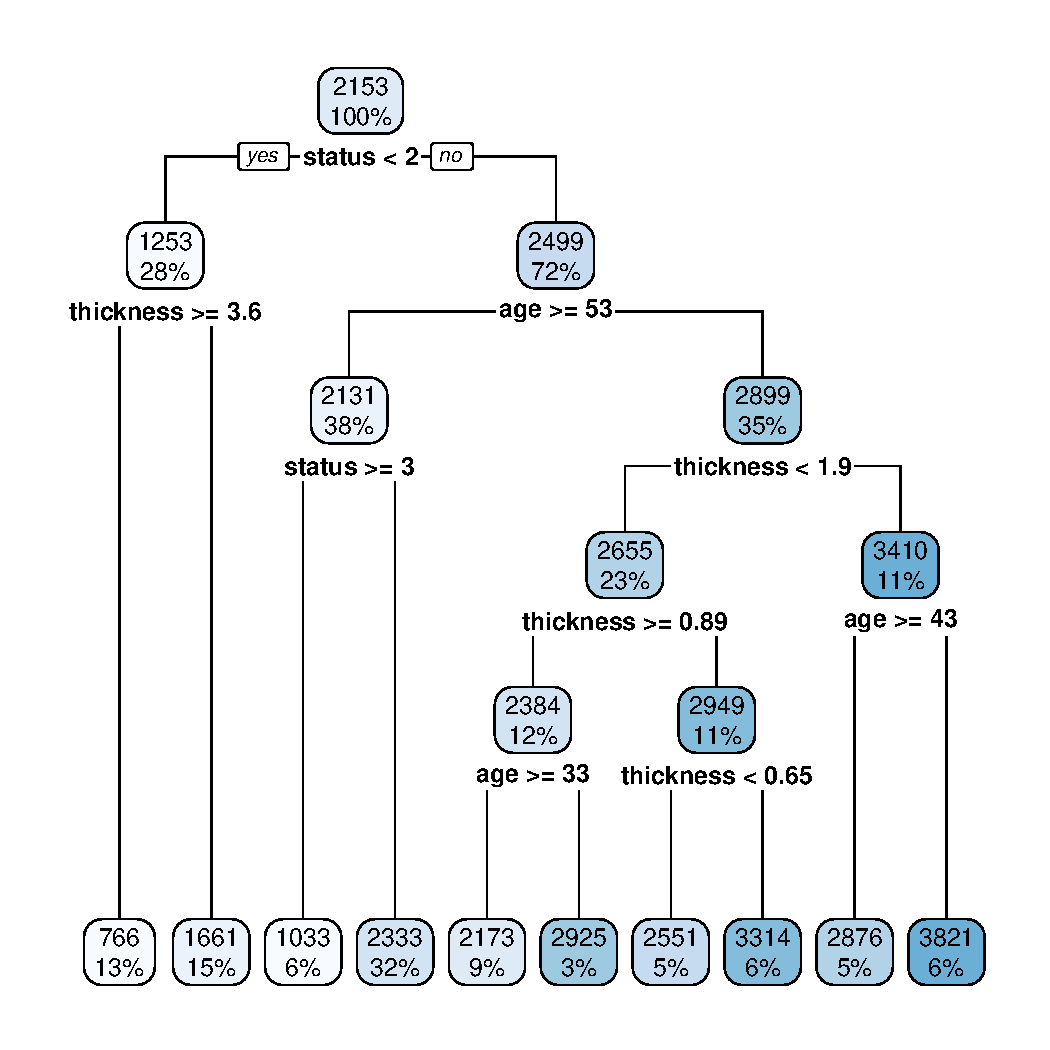
\includegraphics[width = 0.5\textwidth]{rpart_depth6.pdf}
\end{figure} 

\end{frame} 




\begin{frame}
\frametitle{Regularisation: forcing a model to be simpler}
\vspace{-4mm}
\begin{figure}
    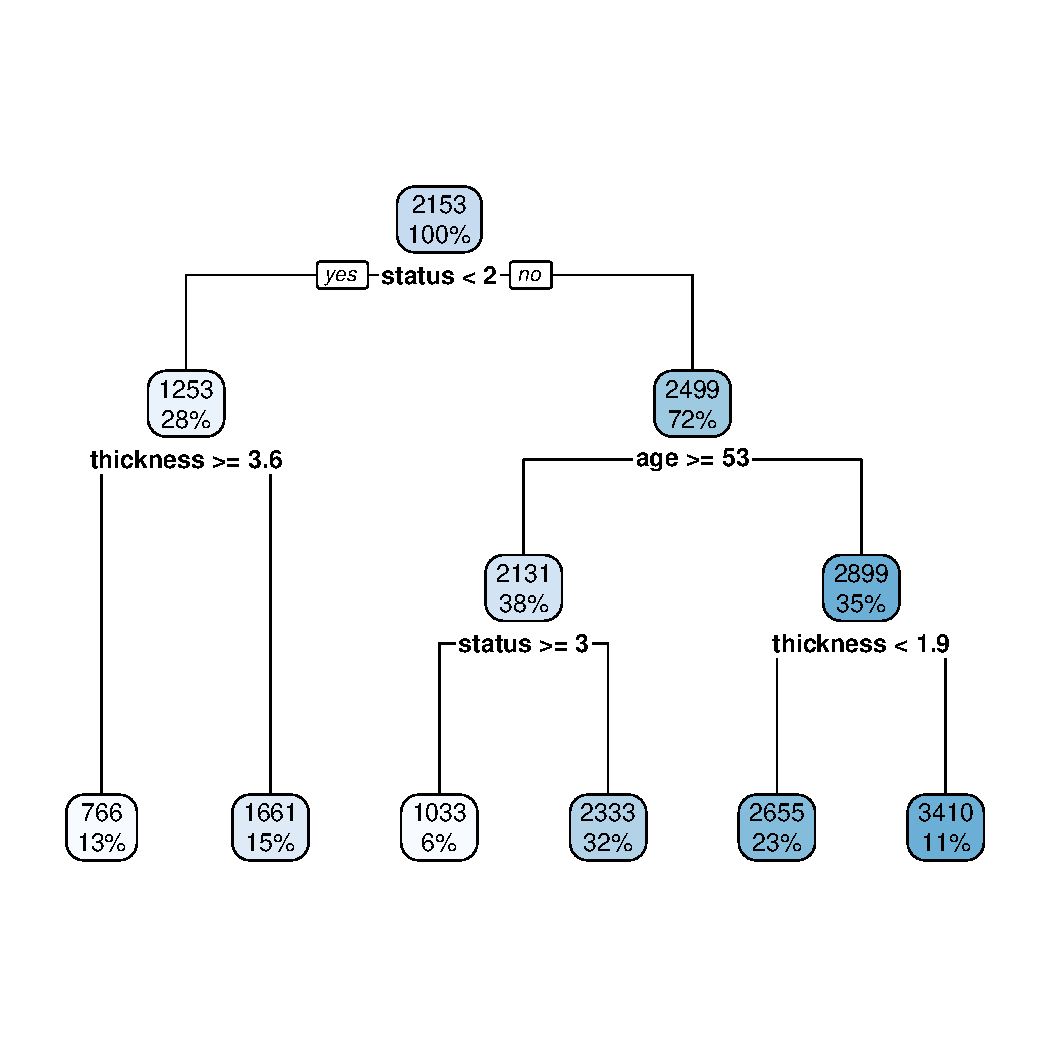
\includegraphics[width = 0.5\textwidth]{rpart_depth3.pdf}
\end{figure} 
\end{frame} 





\begin{frame}
\frametitle{How do we choose? Out-of-sample performance.}
\vspace{-4mm}
\begin{figure}
    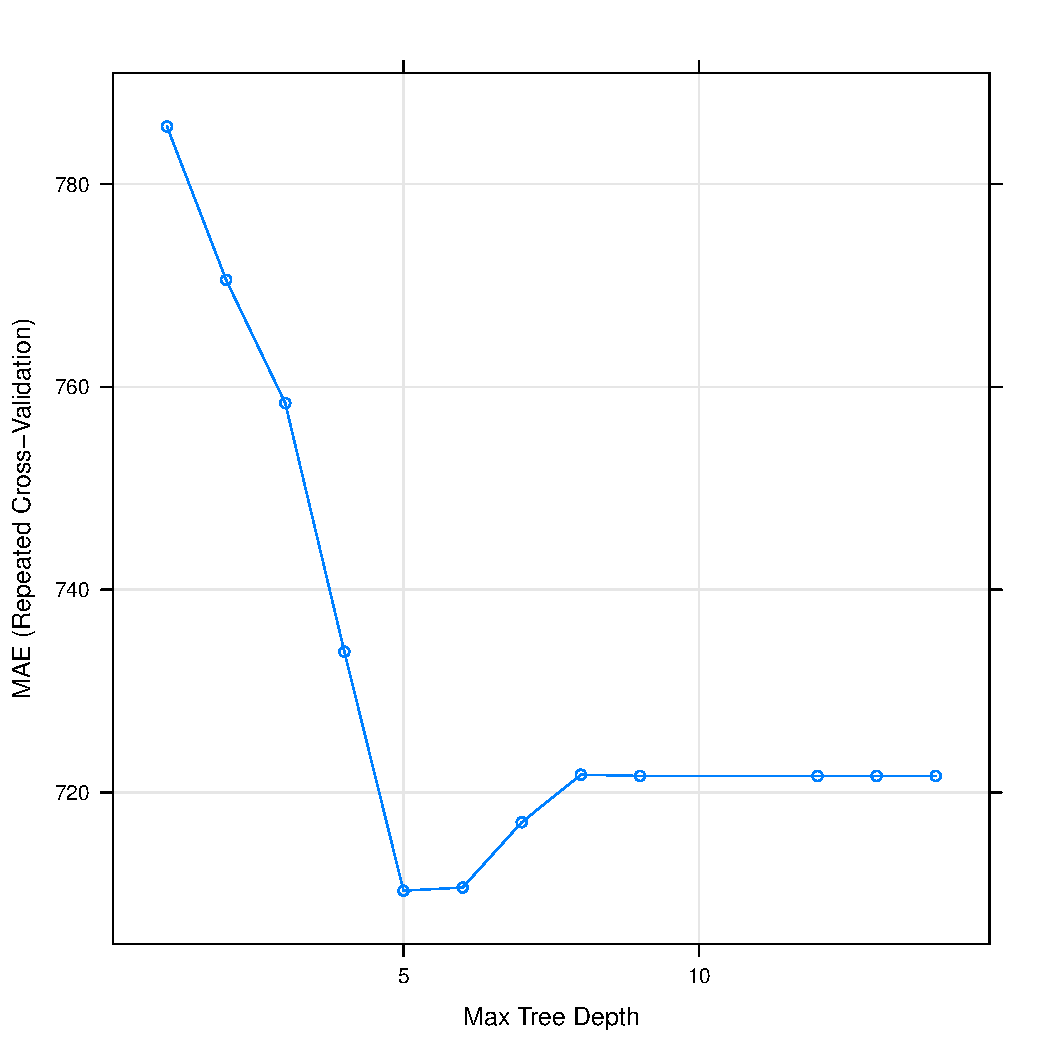
\includegraphics[width = 0.45\textwidth]{rpart_perf.pdf}
\end{figure} 

\end{frame} 


\begin{frame}
\frametitle{Other tuning parameters.}
\begin{itemize}
\item Stepwise regression cutoff.
\item Degree if freedom in GAM
\item Length scale in Gaussian Process
\item Variance of zero-mean Bayesian prior
\end{itemize}

\end{frame} 


\begin{frame}
\frametitle{Why does performance decrease  with model complexity?}
\vspace{-4mm}
\begin{figure}
    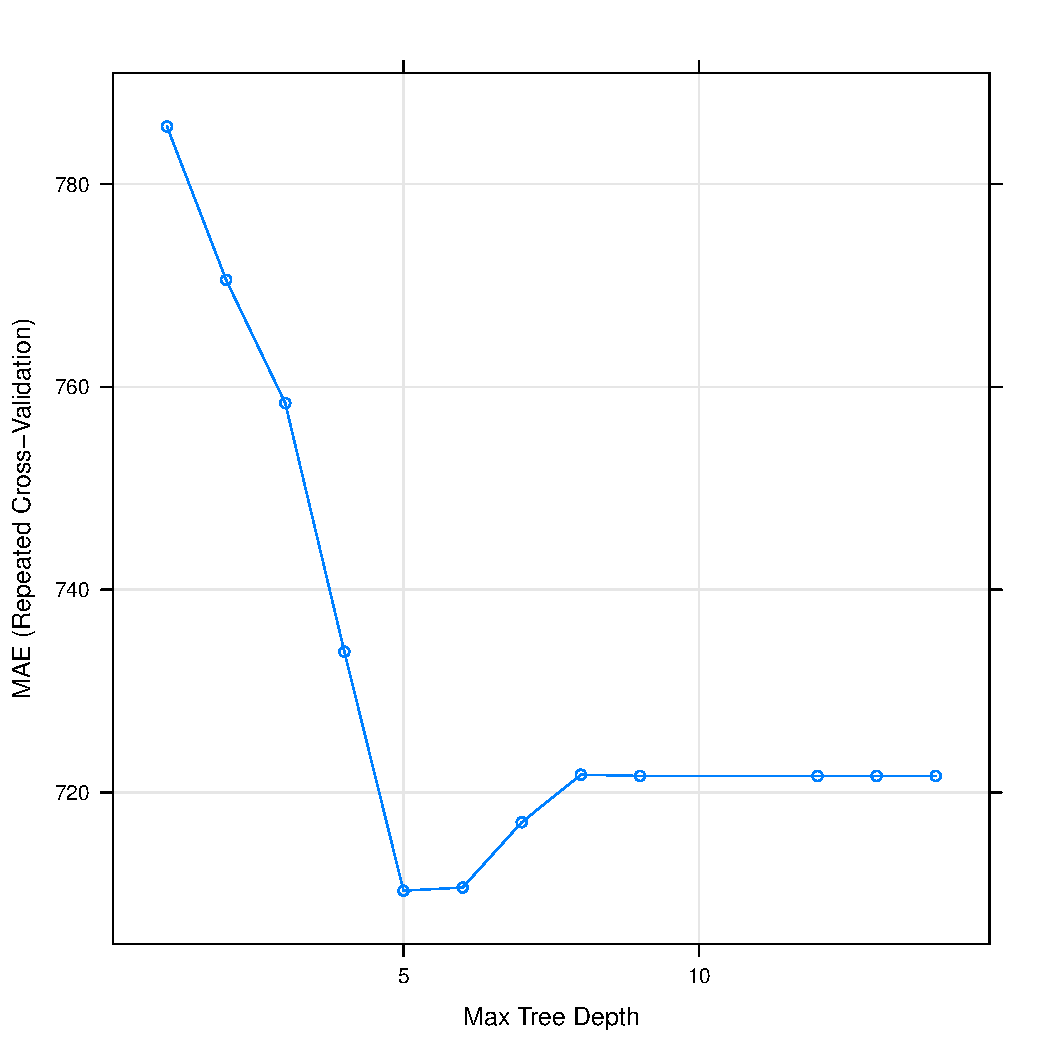
\includegraphics[width = 0.5\textwidth]{rpart_perf.pdf}
\end{figure} 

\end{frame} 


\begin{frame}
\frametitle{Overfitting and bias/variance.}

\begin{figure}
    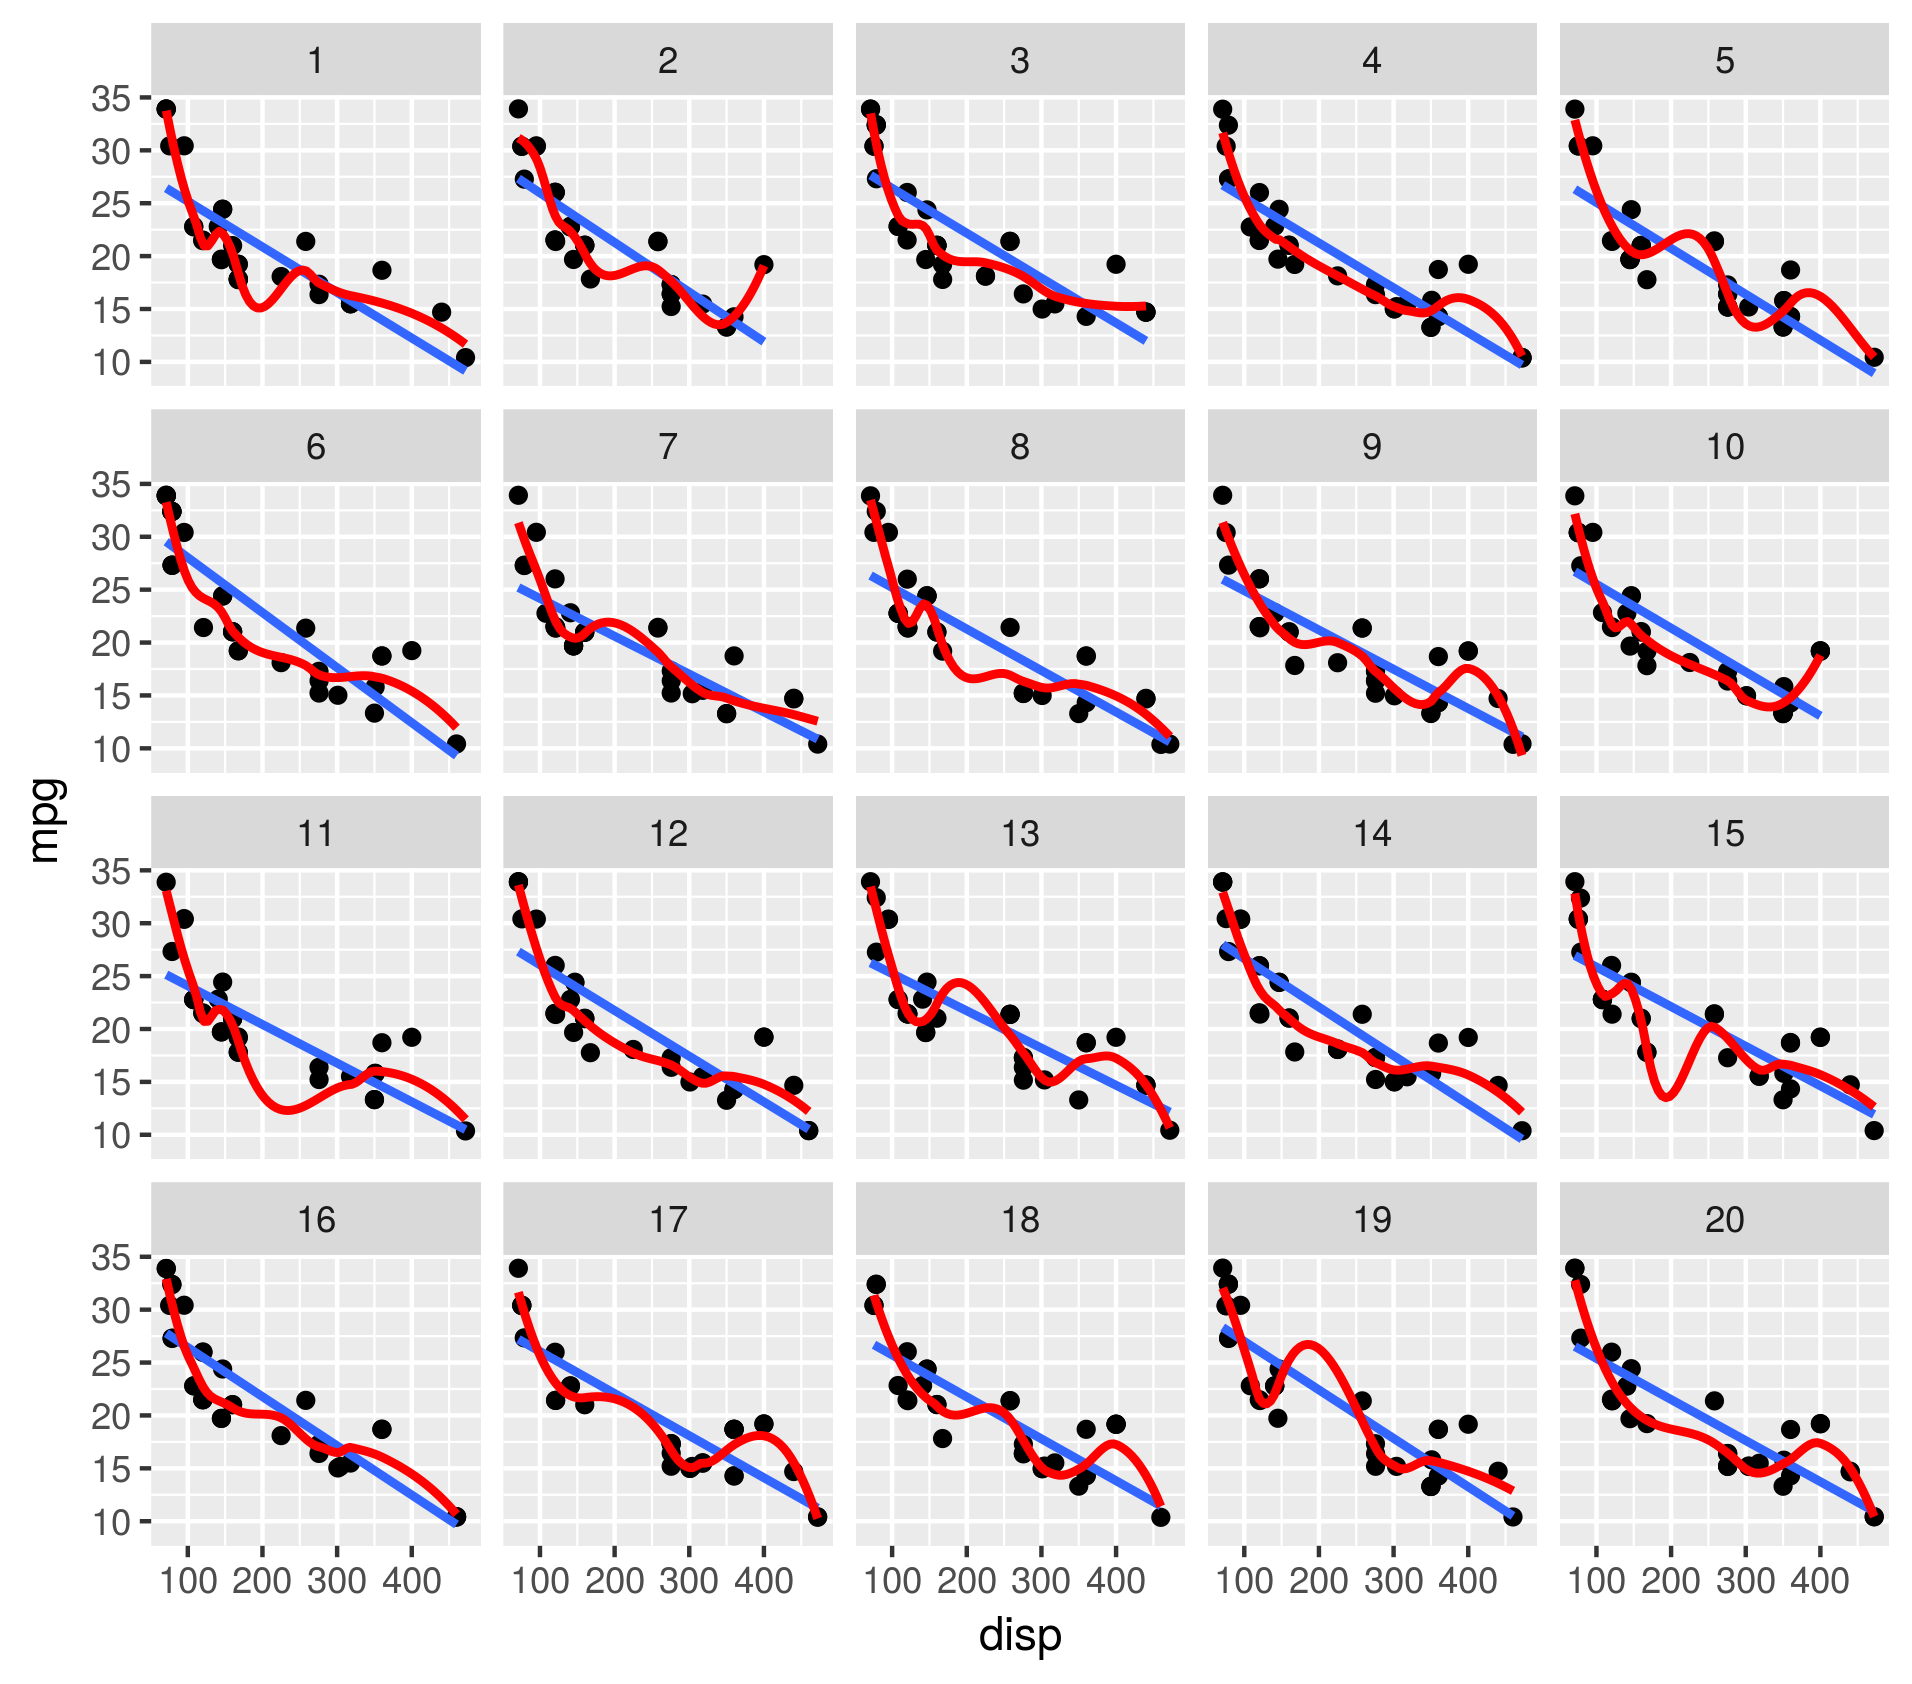
\includegraphics[height = 0.8\textheight]{bias-variance.png}
\end{figure} 

\end{frame} 




\begin{frame}
\frametitle{Any questions?}


\end{frame} 


\begin{frame}[fragile]
\frametitle{Crossvalidation}
\begin{Verbatim}
tr2 <- trainControl(
        method = 'repeatedcv',
        repeats = 3,
        number = 5)

m1 <- train(time ~ ., 
            data = melanoma,
            method = 'rpart2',
            tuneLength = 10,
            metric = 'MAE',
            trControl = tr2)

\end{Verbatim}

\end{frame} 




\begin{frame}
\frametitle{Crossvalidation}

\begin{itemize}
\item k-fold
\begin{itemize}
\item split into k group. user each group on turn as hold out.
\end{itemize}
\item Repeated k-fold
\begin{itemize}
\item Do k-for multiple times with different random splits.
\end{itemize}
\item Bootstrap
\begin{itemize}
\item Sample N with replacement as training.
\end{itemize}
\end{itemize}
\end{frame} 

\begin{frame}
\frametitle{Crossvalidation}

\begin{itemize}
\item Spatial
\item Temporal
\item By covariates
\item What question do you want to ask?
\end{itemize}
\end{frame} 


\begin{frame}
\frametitle{Outer Crossvalidation}

\begin{itemize}
\item Selecting a model \emph{is part of the model}.
\item If we consider many models, taking the best one is a form of overfitting
\item Outer cross-validation of this is part of primary research question.
\item Unfortunately not implemented in caret. Must do it manually.
\end{itemize}
\end{frame} 




\begin{frame}
\frametitle{How noisy is performance?}
\vspace{-4mm}
\begin{figure}
    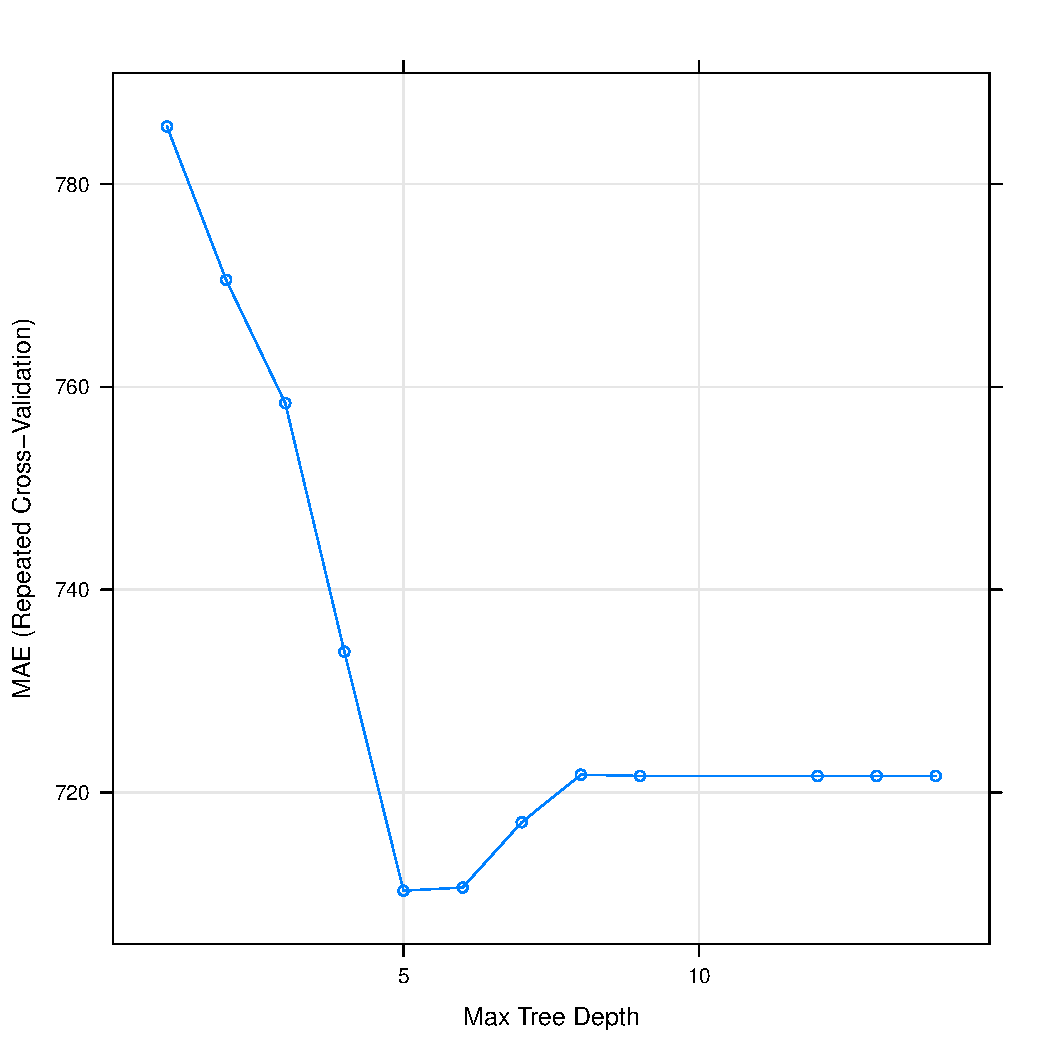
\includegraphics[width = 0.45\textwidth]{rpart_perf.pdf}
\end{figure} 
\end{frame} 






\begin{frame}
\frametitle{Any questions?}


\end{frame} 




\begin{frame}
\frametitle{Error metrics: regression}

\begin{itemize}
\item Match error metric to question.
\item Aim for interpretability.
\item MAE, $R^2$
\item RMSE, correlation are less interpretable
\item Correlation isn't quite measuring what you think.
\end{itemize}
\end{frame} 


\begin{frame}
\frametitle{Error metrics: regression}
\begin{figure}
    \includegraphics[width = 0.8\textwidth]{corr_mae.pdf}
\end{figure} 

\end{frame} 



\begin{frame}
\frametitle{Error metrics: classification}

\begin{itemize}
\item Match error metric to question.
\item Aim for interpretability.
\item Class balance. Model that never predicts rare class will have high accuracy.
\item Kappa, AUC.
\item 
\end{itemize}
\end{frame} 



\begin{frame}
\frametitle{Any questions?}


\end{frame} 



\begin{frame}
\frametitle{No free lunch}
No such thing as a universal, `best' machine learning model.
\end{frame} 




	

\begin{frame}[fragile]
\frametitle{Fuller ML workflow}
\begin{Verbatim}

# Carefully think about hold out data
tr2 <- trainControl(
        method = 'repeatedcv',
        repeats = 3,
        number = 5)

\end{Verbatim}

\end{frame} 


\begin{frame}[fragile]
\frametitle{Fuller ML workflow}
\begin{Verbatim}

# Carefully choose a metric
my_metric <- 'MAE'

\end{Verbatim}

\end{frame} 


\begin{frame}[fragile]
\frametitle{Fuller ML workflow}
\begin{Verbatim}

# Baseline linear model
m1 <- train(time ~ ., 
            data = melanoma,
            method = 'enet',
            tuneLength = 10,
            metric = my_metric,
            trControl = tr2)


# Look at scatter plots for regression
plotCV(m1)

\end{Verbatim}

\end{frame} 



\begin{frame}[fragile]
\frametitle{Fuller ML workflow}
\begin{Verbatim}

# Projection pursuit is very fast but nonlinear.
#   Another good baseline.
m2 <- train(time ~ ., 
            data = melanoma,
            method = 'ppr',
            tuneLength = 10,
            metric = my_metric,
            trControl = tr2)


# Look at scatter plots for regression
plotCV(m2)

\end{Verbatim}

\end{frame} 


\begin{frame}[fragile]
\frametitle{Fuller ML workflow}
\begin{Verbatim}

# Random Forest often peforms well
m3 <- train(time ~ ., 
            data = melanoma,
            method = 'ranger',
            tuneLength = 10,
            metric = my_metric,
            trControl = tr2)


# Look at scatter plots for regression
plotCV(m3)
\end{Verbatim}

\end{frame} 


\begin{frame}[fragile]
\frametitle{Fuller ML workflow}
\begin{Verbatim}

# Consider more complicated models.
m4 <- train(time ~ ., 
            data = melanoma,
            method = 'xgbTree',
            tuneLength = 10,
            metric = my_metric,
            trControl = tr2)

\end{Verbatim}

\end{frame} 



\begin{frame}
\frametitle{Any questions?}


\end{frame} 





\begin{frame}
\frametitle{What is a RandomForest?}

\begin{itemize}
\item Instead of 1 tree, fit many trees and take average prediction.
\item For each tree take a random bootstrap of the data.
\item For each node consider a random subset of covariates.
	\begin{itemize}
	\item Consider mtry covariates. Tuning parameter.
	\end{itemize}
\item These both help prevent overfitting.
\end{itemize}
\end{frame} 


\begin{frame}
\frametitle{What is a Neural Network?}

\vspace{6mm}
\begin{figure}
    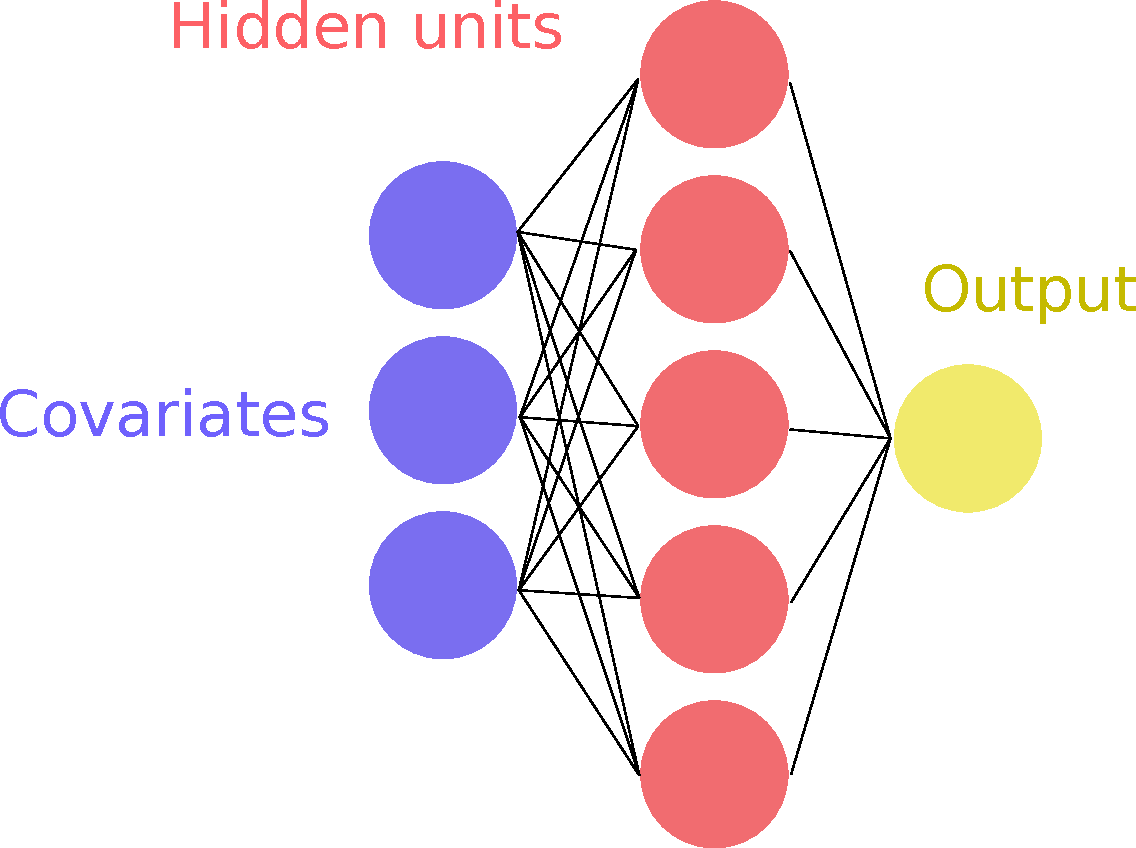
\includegraphics[height = 0.7\textheight]{neural_network.pdf}
\end{figure} 
\end{frame} 


\begin{frame}
\frametitle{What is a Neural Network? Little GLMs.}

\vspace{6mm}
\begin{figure}
    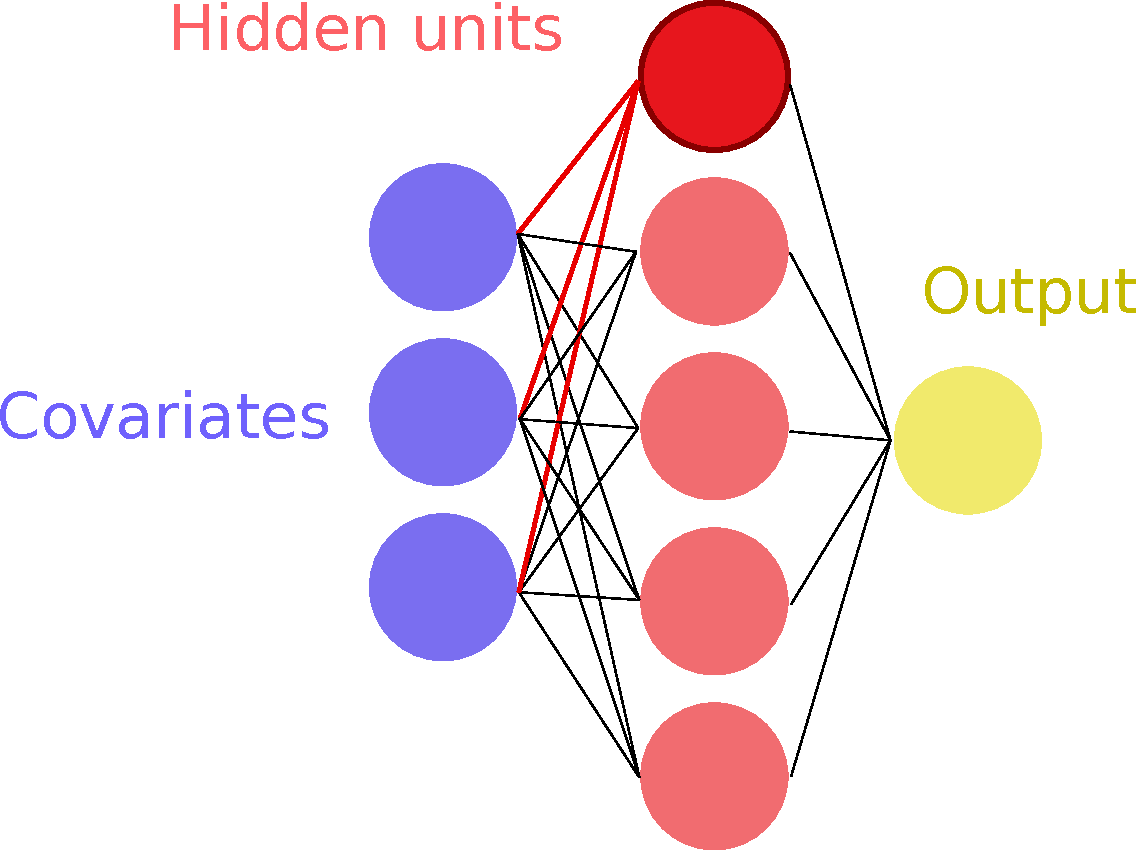
\includegraphics[height = 0.7\textheight]{neural_network2.pdf}
\end{figure} 
\end{frame} 


\begin{frame}
\frametitle{What is a Neural Network? Little GLMs.}

\vspace{6mm}
\begin{figure}
    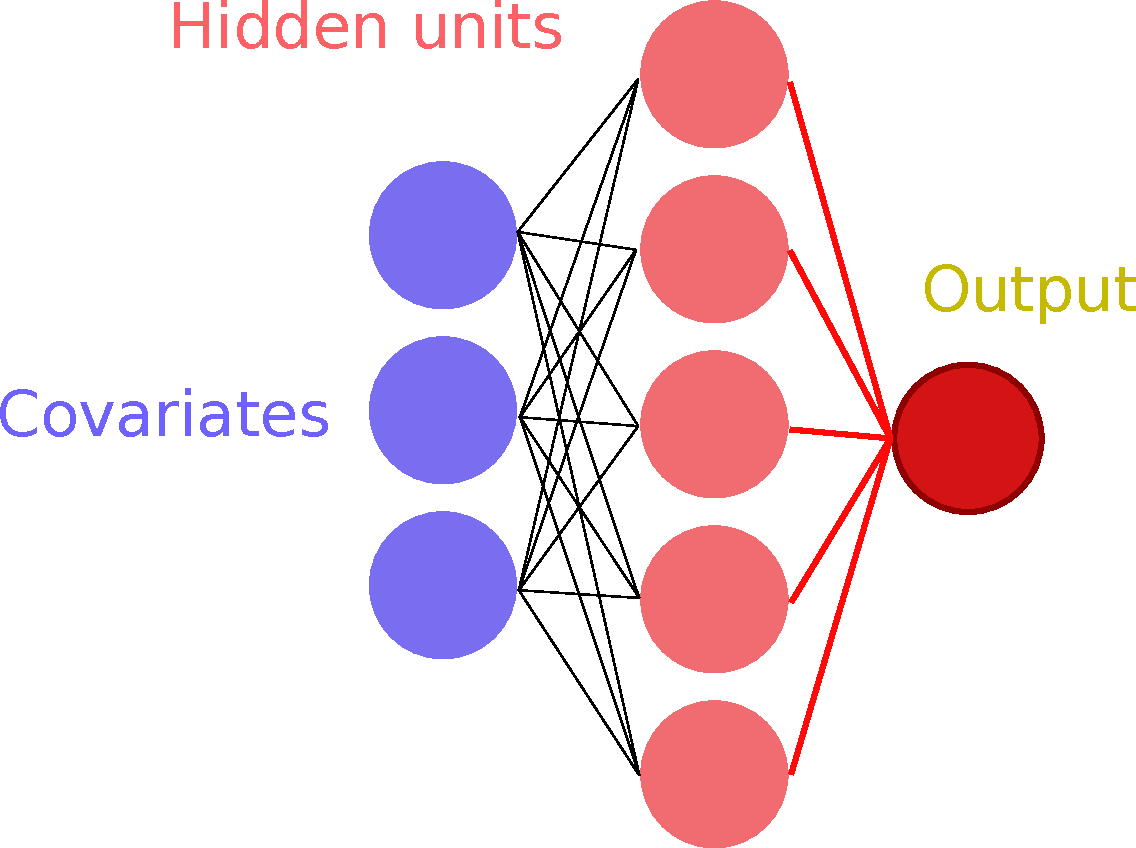
\includegraphics[height = 0.7\textheight]{neural_network3.pdf}
\end{figure} 
\end{frame} 



\begin{frame}
\frametitle{What is a Neural Network?}

\begin{itemize}
\item Optimise the parameters but there are lots of local optima.
\item What ``architecture''?
	\begin{itemize}
	\item Hidden units.
	\item Extra hidden layers
	\item Everything connected to everything else?
	\end{itemize}
\end{itemize}
\end{frame} 




\begin{frame}
\frametitle{Extra reading}

\begin{itemize}
\item Breiman 2001 Statistical Modeling: The Two Cultures.
\item Molnar 2020 Interpretable Machine Learning: A Guide for Making Black Box Models Explainable.
\item Kuhn 2013 Applied Predictive Modeling.
\item Lucas 2020 A translucent box: interpretable machine learning in ecology.
\end{itemize}
\end{frame} 



\begin{frame}
\frametitle{No free lunch}
No such thing as a universal, `best' machine learning model.
\end{frame} 




\begin{frame}

\frametitle{Please ask me some questions}

\vspace{5mm}


\vspace{4mm}


\includegraphics[height=7pt]{Ar_Icon_Contact.pdf} tlucas{\footnotesize{@}}ic.ac.uk


\includegraphics[height=7pt]{Twitter_logo_blue-small.png} {\footnotesize{@}}statsforbios

\vspace{2cm}
\hfill % pushes logo the right
\includegraphics[width=5cm]{../../ceh_logo.png}

\end{frame}


%thanks


 
\end{document}


